
\documentclass[11pt]{beamer}
%Packages
\usepackage{multirow}
\usepackage{graphicx}
\usepackage[utf8]{inputenc}
\usepackage[T1]{fontenc}
\usepackage{aeguill}
\usepackage{amssymb}
\usepackage{pgf,pgfarrows,pgfnodes}
\usepackage[french]{babel}
\usepackage{float}
\usepackage{xkeyval,calc,listings,tikz}
\usepackage{fancyvrb}

%Preamble

\input /Users/remy/cqls/texinputs/Cours/cqlsInclude
\input /Users/remy/cqls/texinputs/Cours/testInclude


\mode<article>{\usepackage{fullpage}}
%\usetheme{Darmstadt}
%\usepackage{times}
%\usefonttheme{structurebold}
\usetheme{Antibes}
%\usecolortheme{lily}

\definecolor{VertFonce}{rgb}{0,.4,.0}

\mode<presentation>
{
  %\usetheme{Warsaw}
  % or ...
\usetheme{Boadilla}

  \setbeamercovered{transparent=5}
  % or whatever (possibly just delete it)
}
%\setbeamercovered{dynamic}


\subject{Talks}

\AtBeginSection[]
{
  \begin{frame}<beamer>
    \frametitle{Plan}
    \tableofcontents[currentsection,currentsubsection]
  \end{frame}
}


\setbeamercovered{invisible}
\newcommand{\Sim}{{\star}}
\newcommand{\ok}{ \textcolor{green}{\large$\surd$}}
\newcommand{\nok}{ \textcolor{red}{\large X}}


\usetikzlibrary{arrows,%
  calc,%
  fit,%
  patterns,%
  plotmarks,%
  shapes.geometric,%
  shapes.misc,%
  shapes.symbols,%
  shapes.arrows,%
  shapes.callouts,%
  shapes.multipart,%
  shapes.gates.logic.US,%
  shapes.gates.logic.IEC,%
  er,%
  automata,%
  backgrounds,%
  chains,%
  topaths,%
  trees,%
  petri,%
  mindmap,%
  matrix,%
  calendar,%
  folding,%
  fadings,%
  through,%
  positioning,%
  scopes,%
  decorations.fractals,%
  decorations.shapes,%
  decorations.text,%
  decorations.pathmorphing,%
  decorations.pathreplacing,%
  decorations.footprints,%
  decorations.markings,%
  shadows}
\tikzset{
  every plot/.style={prefix=plots/pgf-},
  shape example/.style={
    color=black!30,
    draw,
    fill=yellow!30,
    line width=.5cm,
    inner xsep=2.5cm,
    inner ysep=0.5cm}
}

%Styles

%Title


\title[Problématiques Produits A et B]
{Cours de Statistiques Inférentielles}
\author{CQLS~: cqls@upmf-grenoble.fr}
\date{\today}

\begin{document}
\maketitle


%\begin{frame}
%  \titlepage
%\end{frame}
\section{Risque d'erreur de seconde espèce}

\begin{frame}
\frametitle{Définition du risque d'erreur de seconde espèce et objectif}


\begin{exampleblock}{Objectif}
L'analyse du risque d'erreur de seconde espèce permettra de répondre à la question suivante (pour la problématique du produit~A)~: \\ \pause
\begin{center}\color{red}{Avant le jour~J, l'industriel  a-t-il intérêt \\à acheter le jeu de données~?} \pause
\end{center}
\end{exampleblock}

\begin{exampleblock}{Définition du risque d'erreur de seconde espèce}
On rappelle que dans la problématique de l'industriel, deux risques étaient en jeu~: \pause
\begin{enumerate}
\item {\small Risque d'erreur de première espèce~:} \pause {\small \fbox{risque de devenir pauvre} }\pause
\item {\small Risque d'erreur de seconde espèce~:} \pause {\small \fbox{risque de ne pas devenir riche} }
\end{enumerate}
\end{exampleblock}
\end{frame}

\begin{frame}
\frametitle{Risque d'erreur de seconde espèce : généralités}

\begin{exampleblock}{pour tous les paramètres d'intérêt~?}
{\small L'analyse du risque d'erreur de seconde espèce \textbf{ne peut se faire  que} pour des paramètres pour lesquels  la loi de la \textbf{future estimation du paramètre d'intérêt ne dépend que du paramètre d'intérêt} . }\pause
\begin{enumerate}
\item Exemple~: {\color{red} une proportion $p^\Sim$} car (par exemple pour le produit~A), on sait que dans un cadre asymptotique \pause
$$
\Est{p^\Sim}{Y} \SuitApprox \mathcal{N} \left( {\color{blue}p^\Sim} , \sqrt{\frac{{\color{blue}p^\Sim}(1-{\color{blue}p^\Sim)}}{n}  } \right).
$$
\item Contre-exemple~: {\color{red} une moyenne $\mu^\Sim$} car (par exemple pour le produit~B), on sait que dans un cadre asymptotique \pause 
$$
\Est{\mu^\Sim}{Y} \SuitApprox \mathcal{N} \left( {\color{blue}\mu^\Sim} , \sqrt{\frac{{\color{red}\sigma_\Sim^2}}{n}  } \right).
$$
\end{enumerate}
\end{exampleblock}
\end{frame}


\begin{frame}
\frametitle{Retour au produit~A}


\begin{exampleblock}{Objectif plus précis de l'industriel}
Avant le jour~J, l'industriel  a-t-il intérêt à acheter l'échantillon (de taille $n$) \pause 
\textbf{sachant qu' \fbox{a priori}, il pense qu'il y a \fbox{$p^A=19\%$} d'acheteurs potentiels~? \pause et si l'a priori est \fbox{$p^A=17\%$}~?} \pause
\end{exampleblock}


\begin{alertblock}{et encore plus précis}
\pause On va s'intéresser à la question suivante~: \\
\pause Etant donnée la règle de décision fixée à $\alpha=5\%$, si $p^A=19\%$ \textbf{combien} parmi l'infinité des estimations de ce paramètre obtenues avec un échantillon de taille $n=1000$ conduisent \textbf{à ne pas lancer le produit~A}~? 
\end{alertblock}
\end{frame}




\begin{frame}
\frametitle{Evaluation du risque d'erreur de seconde espèce}






\vspace*{-.4cm}
\begin{center}
\only<1-4>{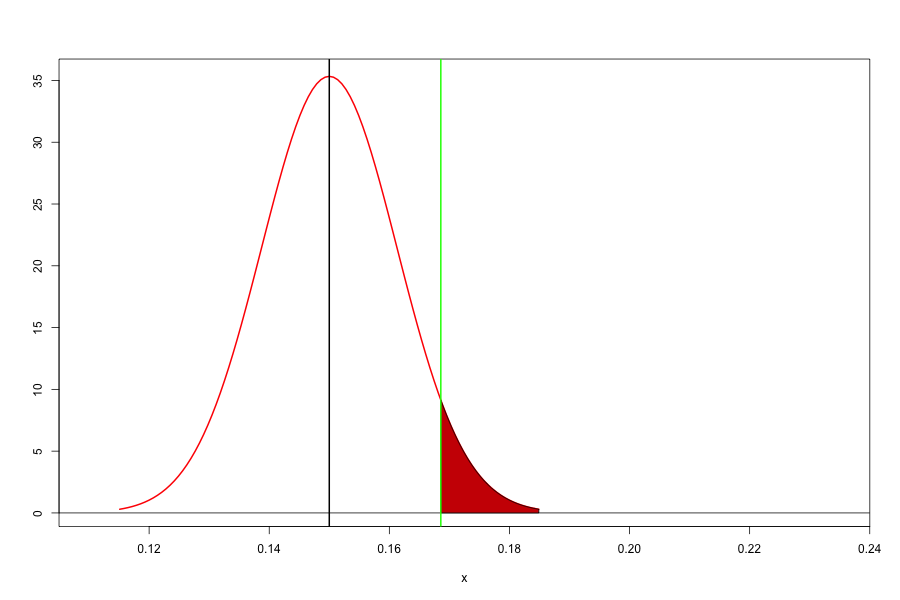
\includegraphics[scale=.25]{img/premEspA}
}\only<5-10>{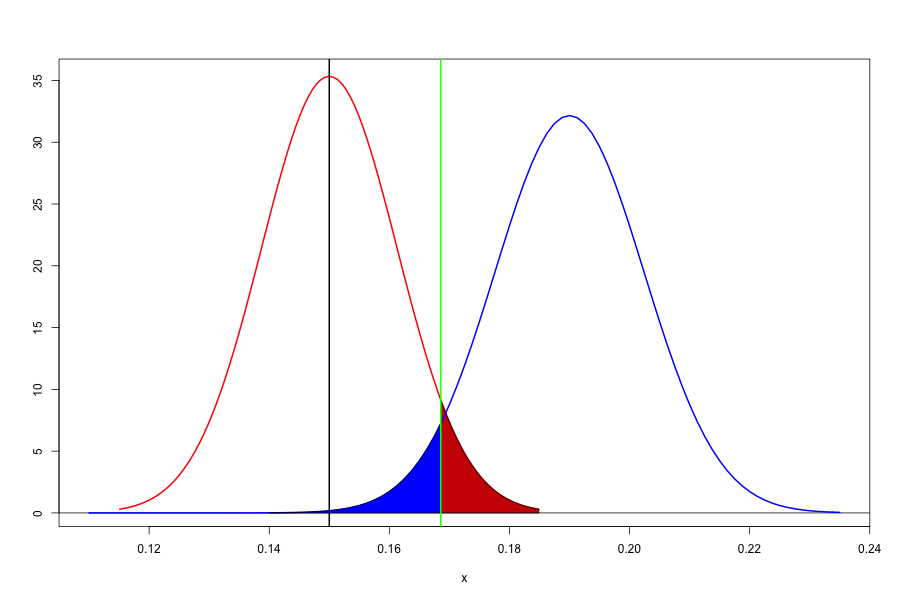
\includegraphics[scale=.25]{img/secEspA19}}
\only<11-12>{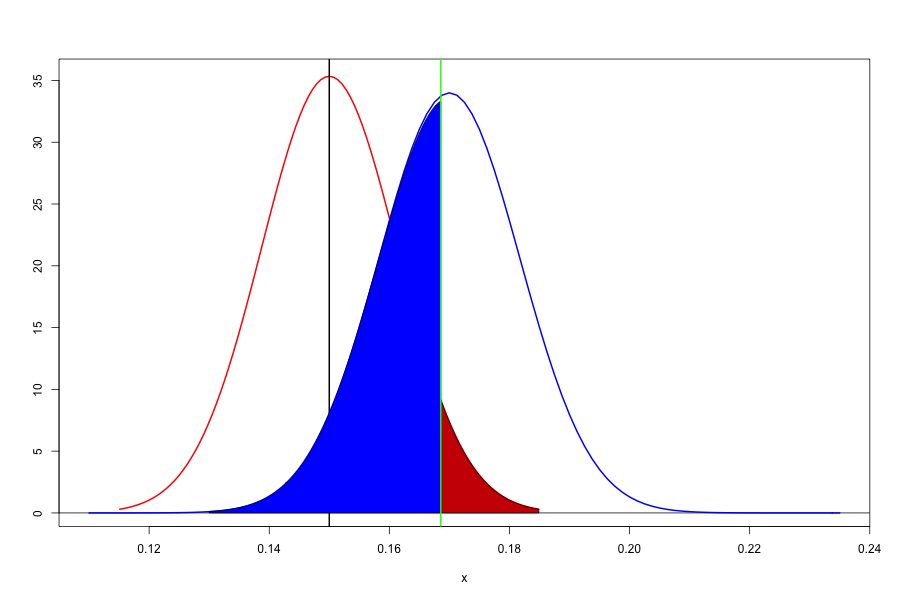
\includegraphics[scale=.25]{img/secEspA17}}
\end{center}



\vspace*{-1cm}

\begin{block}{}
\only<1>{\textbf{Règle de décision :} accepter $\mathbf{H_1}$ si $\Est{p^A}{y^A}>p_{lim,5\%}^+$ avec \\
$p_{lim,5\%}^+ \stackrel{R}{=}$ \texttt{plim =qnorm(.95,.15,sqrt(.15*.85/1000))}}\only<2-3>{\textbf{Question :} comment interpréter la surface rouge par l'A.E.P.~?}\only<3>{\\ \textbf{Réponse :} la proportion parmi l'infinité des estimations de $p^A=15\%$ qui sont supérieures à $p_{lim,5\%}$, i.e. la proportion de ces estimations qui conduisent à lancer le produit A à tort (dans la pire des situations)}\only<4>{\textbf{Question :} comment représenter le tas de toutes les estimations possibles de $p^A=19\%$~?}\only<5-6>{\textbf{Question :} à quoi correspond alors la surface bleue via l'A.E.P}\only<6>{\\ \textbf{Réponse :} à la proportion parmi l'infinité des estimations de $p^A=19\%$ qui sont inférieures à $p_{lim,5\%^+}$, i.e. à la proportion de ces estimations qui conduisent à ne pas lancer le produit A (à tort!)}\only<7-8>{\textbf{Question :} comment définir mathématiquement cette surface~?}\only<8>{\\ \textbf{Réponse :}
$\beta(19\%)= \mathbb{P}_{p^A=19\%}\left( \Est{p^A}{Y^A}<p_{lim,5\%}^+ \right)$}\only<9-10>{\textbf{Question :} conseillez-vous l'industriel d'acheter $\Vect{y^A}$~?}\only<10>{\\ \textbf{Réponse :} puisque
$$\beta(19\%)\stackrel{R}{=} \texttt{pnorm(plim,0.19,sqrt(0.19*0.81/1000))} \simeq 4.2\%$$
est relativement faible, on peut lui conseiller d'acheter $\Vect{y^A}$}
\only<11-12>{\textbf{Question :} et si l'a priori de l'industriel était de $17\%$~?}\only<12>{\\ \textbf{Réponse : }puisque
{\small \begin{eqnarray*}
\beta(17\%)&=& \mathbb{P}_{p^A=17\%}\left( \Est{p^A}{Y^A}<p_{lim,5\%}^+ \right) \\
&\stackrel{R}{=}& \texttt{pnorm(plim,0.17,sqrt(0.17*0.83/1000))} \simeq 45.2\%
\end{eqnarray*}}
est très élevé, on ne lui conseillerait pas d'acheter $\Vect{y^A}$.}
\end{block}
\end{frame}


\begin{frame}
\frametitle{Fonction puissance}

\begin{exampleblock}{plus généralement}
{\small Avant le jour~J, on peut calculer le risque d'erreur de seconde espèce pour tout $p\geq 0.15$ par \pause
\only<1>{\phantom{\centerline{\fbox{$\beta(p) \stackrel{R}{=}$ pnorm(plim,p,sqrt(p*(1-p)/1000)) }}}
}\only<2>{\centerline{\fbox{$\beta(p) = \mathbb{P}_{p^\Sim=p}\left( \Est{p^\Sim}{Y} < p_{lim,5\%}^+\right)$ }}
}\only<3-8>{\centerline{\fbox{$\beta(p) \stackrel{R}{=}$ pnorm(plim,p,sqrt(p*(1-p)/1000)) }} 
} }
\end{exampleblock}

\begin{alertblock}{définition}
\pause \pause {\small Pour tout $0<p<1$, on définit la \textbf{fonction puissance} notée $\gamma(p)$. Cette quantité représente les chances que l'on a si \fbox{$p^\Sim=p$} de lancer le produit~A (si la règle de décision est fixée à $\alpha=5\%$), i.e. 
\centerline{\fbox{$\gamma(p) = \mathbb{P}_{p^\Sim=p}\left( \Est{p^\Sim}{Y} > p_{lim,5\%}^+\right)$}}
 }
\pause
{\small \begin{enumerate}
\item lorsque $p<0.15$, \pause \fbox{$\gamma(p)=$ risque de devenir pauvre si $p^\Sim=p$.} \pause
\item lorsque $p\geq0.15$~? \pause \fbox{ $\gamma(p)=1-\beta(p)$}
\end{enumerate}}
\end{alertblock}

\end{frame}

\begin{frame}
\frametitle{La fonction puissance en image}






\begin{center}
\only<1>{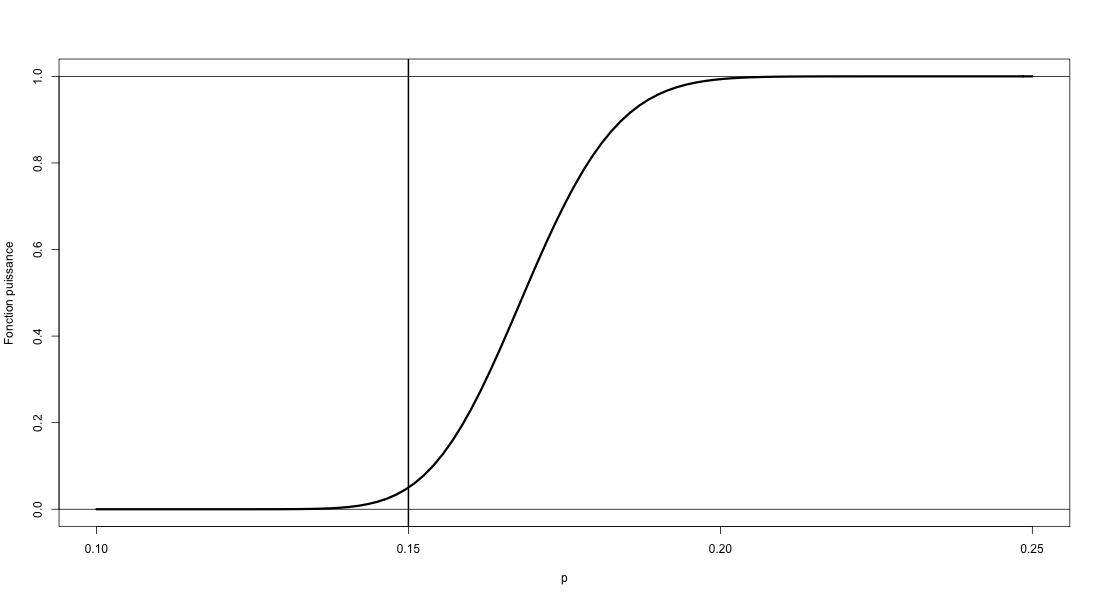
\includegraphics[scale=.25]{img/fctPuiss}
}\only<2>{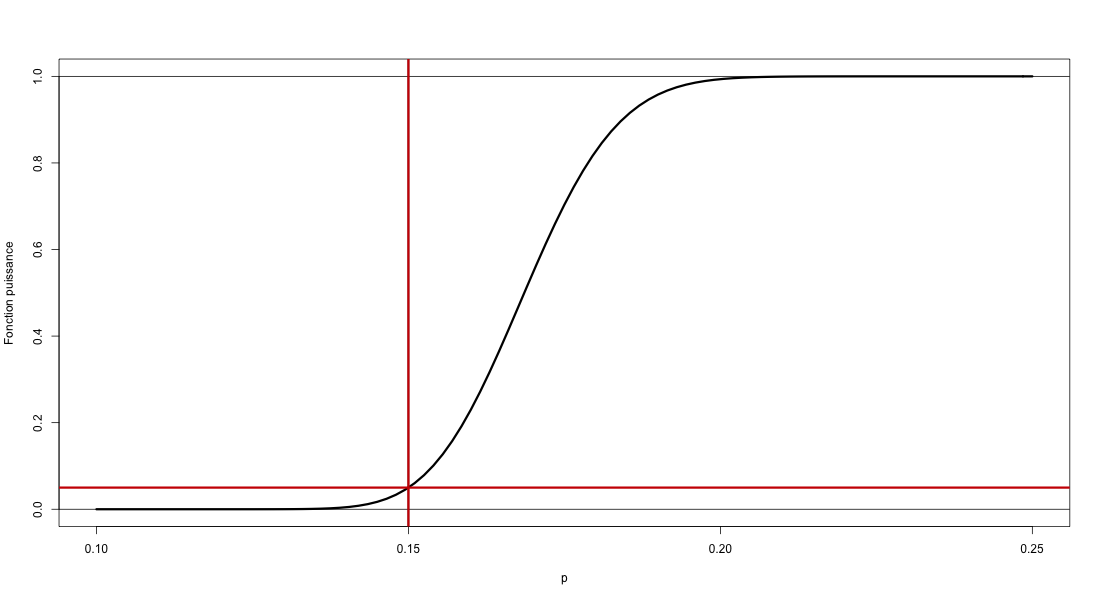
\includegraphics[scale=.25]{img/fctPuiss15}
}\only<3>{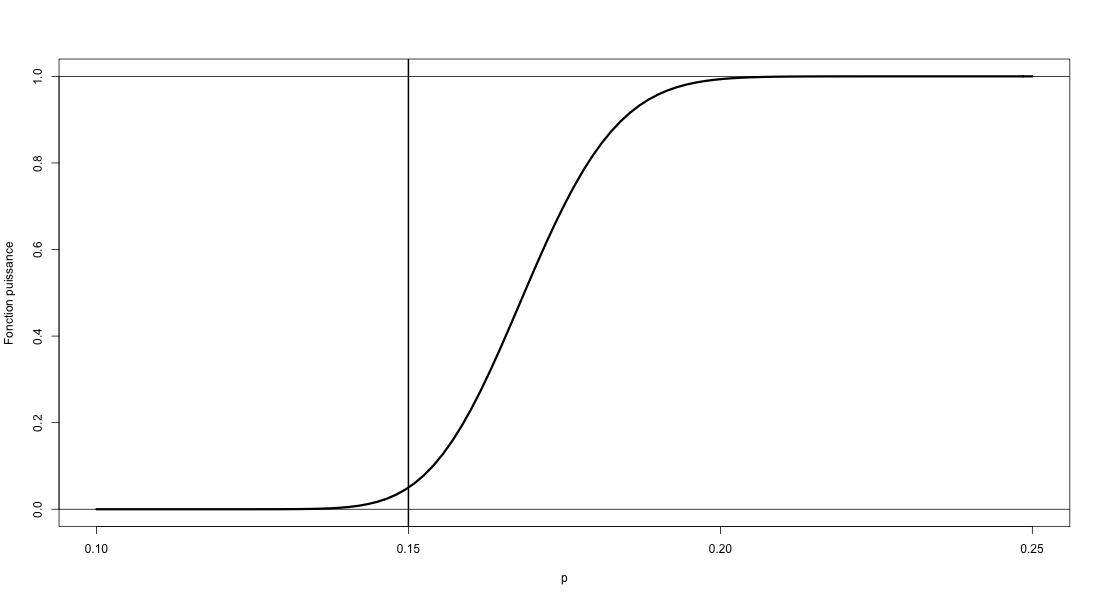
\includegraphics[scale=.25]{img/fctPuiss}
}\only<4>{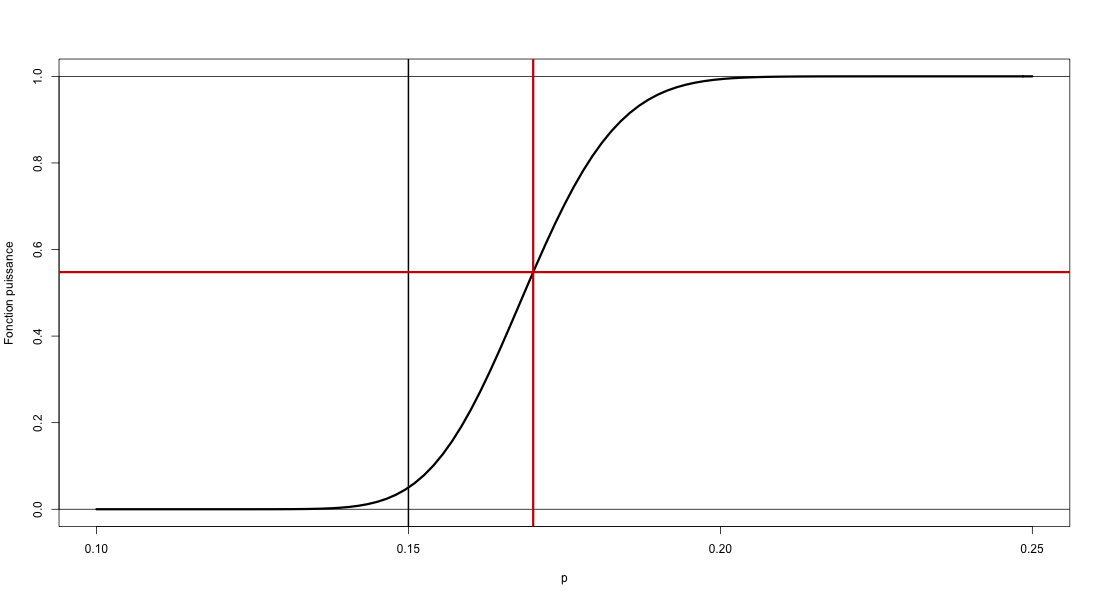
\includegraphics[scale=.25]{img/fctPuiss17}
}\only<5>{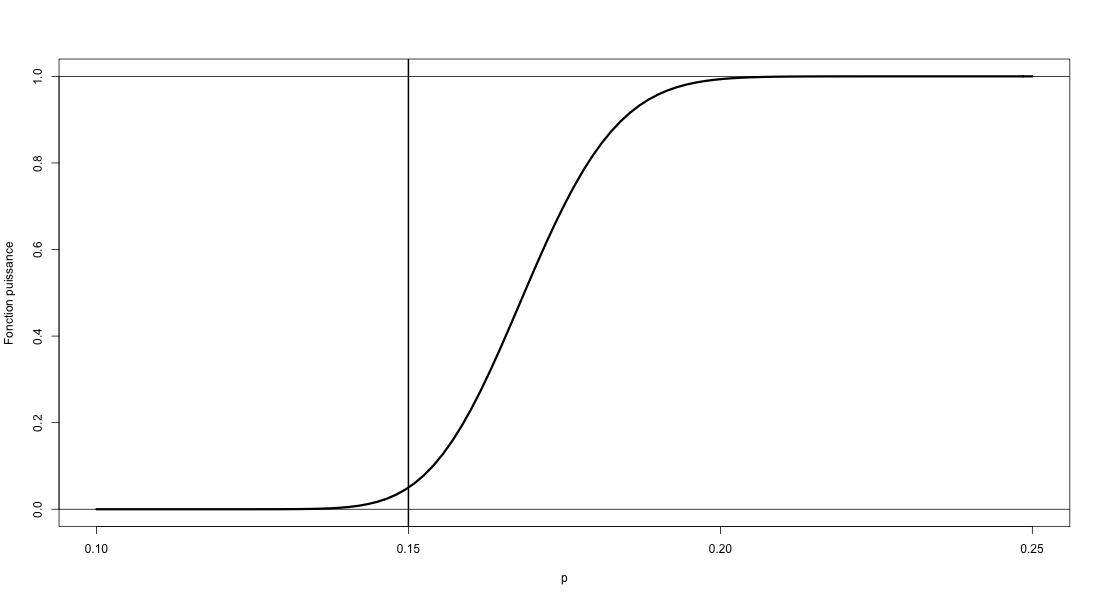
\includegraphics[scale=.25]{img/fctPuiss}
}\only<6>{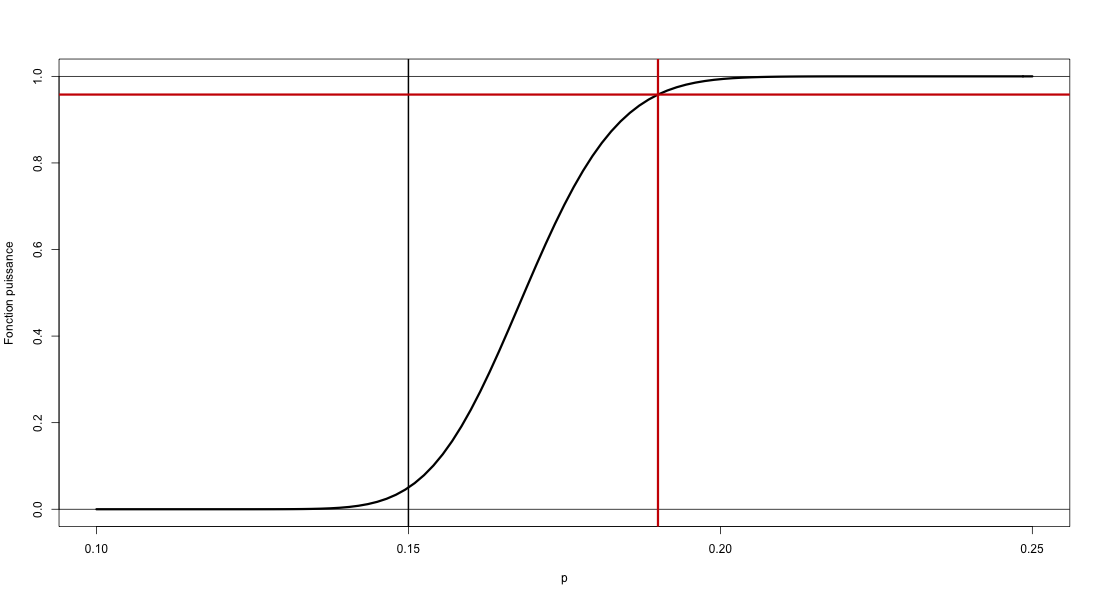
\includegraphics[scale=.25]{img/fctPuiss19}
}
\end{center}

\begin{block}{Questions}
Que vaut 
\only<1>{$\gamma(15\%)$~?
}\only<2>{$\gamma(15\%)$~? {\color{red}Réponse : \fbox{5\%}}
}\only<3>{$\gamma(17\%)$~?
}\only<4>{$\gamma(17\%)$~? {\color{red}Réponse : $\gamma(17\%)=1-\beta(17\%)\simeq 55\%$}
}\only<5>{$\gamma(19\%)$~?
}\only<6>{$\gamma(19\%)$~? {\color{red}Réponse : $\gamma(19\%)=1-\beta(19\%)\simeq 4\%$}
}
\end{block}

\end{frame}

\begin{frame}
\frametitle{Choix de la taille d'échantillon}

\begin{block}{les contraintes de l'industriel}
L'industriel souhaite construire une règle de décision avec un risque de devenir pauvre $\alpha=5\%$ et pense qu'a priori son produit sera acheté par au moins 17\% d'acheteur potentiels. \pause

Comment \textbf{ajuster la taille d'échantillon} de telle sorte que $\alpha=5\%$ et $\beta(17\%)\leq 5\%$~?
\end{block}
\pause 
\begin{alertblock}{Merci qui~? le matheux évidemment }
Le mathématicien nous dit qu'il suffit de prendre $n$ tel que \\
\centerline{\fbox{
${\displaystyle  n \geq \left( \frac{ q_{ 1-\alpha }\times \sqrt{0.15(1-0.15)} + q_{\beta(17\%)}  \times \sqrt{0.17(1-0.17)}          }{17\% - 15 \%}  \right)^2}$
}}

\pause  Application en R~: il faut que \textbf{$n\geq$ 3632.0 }  
\end{alertblock}

\end{frame}

\begin{frame}
\frametitle{Choix de la taille d'échantillon}

\begin{block}{les contraintes de l'industriel}
L'industriel souhaite construire une règle de décision avec un risque de devenir pauvre $\alpha=5\%$ et pense qu'a priori son produit sera acheté par au moins 19\% d'acheteur potentiels. \pause

Comment \textbf{ajuster la taille d'échantillon} de telle sorte que $\alpha=5\%$ et $\beta(19\%)\leq 5\%$~?
\end{block}
\pause 
\begin{alertblock}{Merci qui~? le matheux évidemment }
Le mathématicien nous dit qu'il suffit de prendre $n$ tel que \\
\centerline{\fbox{
${\displaystyle  n \geq \left( \frac{ q_{ 1-\alpha }\times \sqrt{0.15(1-0.15)} + q_{\beta(19\%)}  \times \sqrt{0.19(1-0.81)}          }{19\% - 15 \%}  \right)^2}$
}}

\pause  Application en R~: il faut que \textbf{$n\geq$ 950.0 }  
\end{alertblock}

\end{frame}




\end{document}


